\begin{pastexam}[label={px:ccu-115-swa-08}]{中正資工所甲組 115 學年度 第 18 題}
（複選；全對才給分）

(2\%) (\qquad) What are the output values of $low(v)$ for each vertex $v$ in the given graph, listed
in the order of $A, B, C, D, E, F, G, H,$ and $I$, when determining the articulation points in the
graph from the previous question?

（前一題：For determining the articulation points in the following graph, list the depth-first search
numbers (starting from 1) for each vertex in the order of $A, B, C, D, E, F, G, H,$ and $I$. Begin
the depth-first search at \textbf{vertex $A$}. If multiple unvisited vertices are available during
the search, select the vertex with the smallest alphabetical label.）
\begin{center}
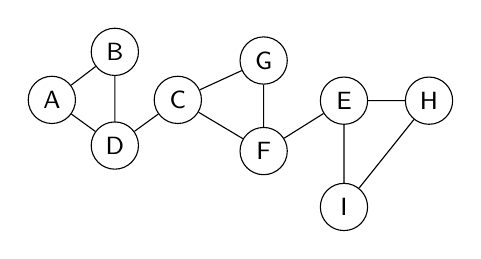
\begin{tikzpicture}[x=1cm,y=1cm,v/.style={circle,draw,minimum size=6mm,inner sep=1pt,font=\small\sffamily}]
\node[v] (A) at (0.75,-1.17) {A};
\node[v] (B) at (1.55,-0.56) {B};
\node[v] (D) at (1.55,-1.75) {D};
\node[v] (C) at (2.35,-1.17) {C};
\node[v] (G) at (3.44,-0.67) {G};
\node[v] (F) at (3.44,-1.82) {F};
\node[v] (E) at (4.46,-1.18) {E};
\node[v] (H) at (5.54,-1.18) {H};
\node[v] (I) at (4.46,-2.53) {I};
\draw (A)--(B) (A)--(D) (B)--(D) (D)--(C) (C)--(G) (C)--(F) (G)--(F) (F)--(E) (E)--(H) (E)--(I) (H)--(I);
\end{tikzpicture}
\end{center}
(a)~(1, 2, 4, 3, 6, 4, 4, 6, 6) \qquad (b)~(1, 1, 4, 1, 6, 5, 9, 6, 6)\\
(c)~(1, 1, 4, 1, 6, 4, 4, 7, 8) \qquad (d)~(1, 1, 4, 1, 6, 4, 4, 6, 6)\\
(e)~none of the above
\end{pastexam}

\begin{pastsoln}
答案：(d)。

$d$ 值和 DFS 樹用前一題（歷屆試題~\ref{px:ccu-115-swa-07}）的結果：$d$ 依 A--I 是
$(1, 2, 4, 3, 6, 5, 9, 7, 8)$；樹邊 A--B、B--D、D--C、C--F、F--E、E--H、H--I、F--G，後向邊 D--A、G--C、I--E。

$\mathit{low}[u]$ 是 $d[u]$、各子節點的 $\mathit{low}$、$u$ 的後向邊另一端的 $d$ 三者的最小值
（資結書第~23.5~節）。 從葉節點往上算：
\begin{center}
\small
\begin{tabular}{cccccc}
\toprule
$u$ & $d[u]$ & 子節點 & 後向邊到 & $\mathit{low}[u]$ \\
\midrule
I & 8 & — & E（$d = 6$） & $\min(8, 6) = 6$ \\
H & 7 & I & — & $\min(7, 6) = 6$ \\
E & 6 & H & — & $\min(6, 6) = 6$ \\
G & 9 & — & C（$d = 4$） & $\min(9, 4) = 4$ \\
F & 5 & E, G & — & $\min(5, 6, 4) = 4$ \\
C & 4 & F & — & $\min(4, 4) = 4$ \\
D & 3 & C & A（$d = 1$） & $\min(3, 4, 1) = 1$ \\
B & 2 & D & — & $\min(2, 1) = 1$ \\
A & 1 & B & — & $1$ \\
\bottomrule
\end{tabular}
\end{center}
依 A--I 的順序：$(1, 1, 4, 1, 6, 4, 4, 6, 6)$，就是 (d)。 （後向邊在兩端都看得到，例如 A 看到 D；
但對祖先那一端，另一端的 $d$ 比自己大，不影響最小值，表裡只列子孫那一端。）
\begin{itemize}
\item (a) 錯：$\mathit{low}[B] = 2$、$\mathit{low}[D] = 3$ 漏了後向邊 D--A。
\item (b) 錯：$\mathit{low}[F] = 5$、$\mathit{low}[G] = 9$ 漏了後向邊 G--C。
\item (c) 錯：$\mathit{low}[H] = 7$、$\mathit{low}[I] = 8$ 漏了後向邊 I--E。
\item (e) 錯，(d) 對。
\end{itemize}
\end{pastsoln}
